\begin{enumerate}[label=\thesubsection.\arabic*.,ref=\thesubsection.\theenumi]
\numberwithin{equation}{enumi}
\numberwithin{figure}{enumi}
\item $\vec{D}_1$ is a point on $BC$ such that
		\begin{align}
			AD_1 \perp BC
		\end{align}
		and $AD_1$ is defined to be the altitude. 
		Find the normal vector of $AD_1$.
  \\
		\solution
The normal vector of $AD_{1}$ 
is
the direction vector $BC$ and is obtained from  
		\eqref{eq:app-geo-dir-vec-bc}
		as
\begin{align}
	\vec{n} = 
\myvec{1\\-11}
\end{align}


	\item Find the equation of $AD_1$.
 \\     \solution
The equation of $AD_1$ is
\begin{align}
 \vec{n}^{\top}(\vec{x-A}) &= 0 \\
\implies \myvec{-1 & 11}\vec{x} &= \myvec{-1 & 11}\myvec{1 \\ -1}
= -12
\end{align}


	\item Find the equations of the altitudes $BE_1$ and $CF_1$ to the sides $AC$ and $AB$ respectively. 
  \\     \\ \solution
\begin{enumerate}
\item 
	From 
		\eqref{eq:app-geo-dir-vec-ca},
the normal vector of $CF_1$ is 
\begin{align}
\vec{n}&=\myvec{-5\\7} 
\end{align}
and the equation of $CF_1$ is
\begin{align}
\vec{n}^{\top}\brak{\vec{x}-\vec{C}}&=0 \\
\implies 
\myvec{-5 & 7}\brak{\vec{x}-\myvec{-3\\-5}}&=0  \\
	\implies \myvec{5 & -7}\vec{x}&=20
		\label{eq:app-geo-alt-cf},
\end{align}
\item Similarly, 
	from 
		\eqref{eq:app-geo-dir-vec-ab},
the normal vector of $BE_1$ is 
\begin{align}
\vec{n}= \myvec{1 \\1}
\end{align}
and the equation of  $BE_1$ is
\begin{align}
\vec{n}^{\top}\brak{\vec{x}-\vec{B}}&=0 \\
	\implies \myvec{1 & 1}\brak{\vec{x}-\myvec{-4\\6}}&=0 \\
	\implies \myvec{1 & 1}\vec{x}&=2
		\label{eq:app-geo-alt-be},
\end{align}
\end{enumerate}



	\item Find the intersection $\vec{H}$ of $BE_1$ and $CF_1$.
 \\
        \\ \solution
%
The intersection of 
		\eqref{eq:app-geo-alt-be}
		and
		\eqref{eq:app-geo-alt-cf},
		is obtained from 
		the matrix equation
		%
\begin{align}
        \myvec{1&1\\5&-7} \vec{x} &= \myvec{2\\20}
\end{align}
%
which can be solved as 
%
\begin{align}
        \myvec{1&1&2\\5&-7&20}
	 \xleftrightarrow[]{R_2 \leftarrow R_2 - 5R_1}
        \myvec{1&1&2\\0&-12&10}\\
	 \xleftrightarrow[]{R_2 \leftarrow \frac{R_2}{-12}}
        \myvec{1&1&2\\0&1&\frac{-5}{6}}
	 \xleftrightarrow[]{R_1 \leftarrow R_1 - R_2}
        \myvec{1&0&\frac{17}{6}\\0&1&\frac{-5}{6}}
\end{align}
%
yielding
%
\begin{align}
        \vec{H}&=\frac{1}{6}\myvec{{17}\\-{5}}
		\label{eq:app-geo-alt-H},
\end{align}
%
See 
\figref{fig:m_tri_py}
\begin{figure}[H]
\centering
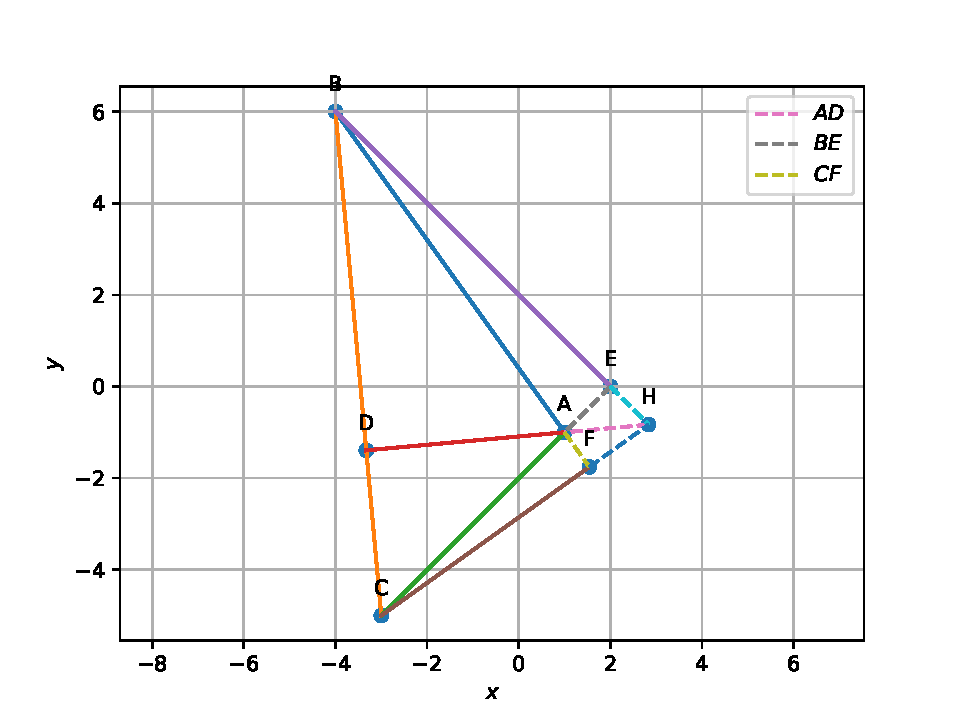
\includegraphics[width=0.75\columnwidth]{figs/triangle/altitude.pdf}
\caption{Altitudes $BE_1$ and $CF_1$ intersect at $\vec{H}$}
\label{fig:m_tri_py}
\end{figure}


	\item Verify that 
		\begin{align}
			\brak{\vec{A}-\vec{H}}^{\top}\brak{\vec{B}-\vec{C}} = 0
		\end{align}
  \solution
From 
		\eqref{eq:app-geo-alt-H},
\begin{align}
\vec{A}-\vec{H}=-\frac{1}{6}\myvec{{11}\\{1}},\,
\vec{B}-\vec{C}=\myvec{-1\\11}
\\
	\implies \brak{\vec{A}-\vec{H}}^{\top}\brak{\vec{B}-\vec{C}}=\frac{1}{6}\myvec{11 & 1}
\myvec{-1\\11}
=0
\end{align}


  \item Find the length of the altitude $AD_1$.
	  \\
		\solution 
		If the equation of $BC$ be $\vec{n}^\top\vec{x} =c$,
%from
		%	\eqref{eq:geo-param},
\begin{align}
			\label{eq:app-geo-param-app}
	\vec{D}_1 = \vec{A} + k\vec{n}
	\\
	\implies AD_1 = \norm{\vec{D}_1 - \vec{A}}=\abs{k} \norm{\vec{n}}
			\label{eq:app-geo-param-app-PQ}
\end{align}
			From \eqref{eq:app-geo-param-app},
\begin{align}
	\vec{n}^{\top}  \vec{D}_1 = \vec{n}^{\top}  \vec{A} + k\norm{\vec{n}}^2
	\\
	\implies \abs{k} = 
	\frac{\abs{\vec{n}^{\top}\brak{\vec{D}_1 - \vec{A}}}}{\norm{\vec{n}}^2}
			\label{eq:app-geo-param-app-k}
			\\
	\implies AD_1 =\abs{k}  
		\norm{\vec{n}}	=
	\frac{\abs{\vec{n}^{\top}\vec{A} - c}}{\norm{\vec{n}}}
			\label{eq:app-PQ-final}
\end{align}
upon substituting from 
			\eqref{eq:app-geo-param-app-PQ}.
  \item Find $\vec{D}_1$.
	  \\
		\solution $\because \vec{D}_1$ lies on $BC$, 
\begin{align}
			\label{eq:app-BC-alt}
\vec{n}^\top\vec{D}_1 =c
\end{align}
and 
	$\because AD_1 \perp BC$,
\begin{align}
	\vec{m}^{\top}\brak{\vec{A}-\vec{D}_1} = 0
	\\
	\implies 
	\vec{m}^{\top}\vec{D}_1 = 
	\vec{m}^{\top}\vec{A}
			\label{eq:app-AD1-alt}
\end{align}
Clubbing
			\eqref{eq:app-BC-alt}
			and 
			\eqref{eq:app-AD1-alt},
\begin{align}
			\label{eq:app-D1-alt}
	\myvec{\vec{m} & \vec{n}}^\top\vec{D}_1 &= 
	   \myvec{
              \vec{m}^\top\vec{A}\\
	      c
	      }
\end{align}
\item 
The code for finding the altitude is available at
\begin{lstlisting}
	codes/msoft/altitude.c
\end{lstlisting}
\end{enumerate}
